\documentclass[1p]{elsarticle_modified}
%\bibliographystyle{elsarticle-num}

%\usepackage[colorlinks]{hyperref}
%\usepackage{abbrmath_seonhwa} %\Abb, \Ascr, \Acal ,\Abf, \Afrak
\usepackage{amsfonts}
\usepackage{amssymb}
\usepackage{amsmath}
\usepackage{amsthm}
\usepackage{scalefnt}
\usepackage{amsbsy}
\usepackage{kotex}
\usepackage{caption}
\usepackage{subfig}
\usepackage{color}
\usepackage{graphicx}
\usepackage{xcolor} %% white, black, red, green, blue, cyan, magenta, yellow
\usepackage{float}
\usepackage{setspace}
\usepackage{hyperref}

\usepackage{tikz}
\usetikzlibrary{arrows}

\usepackage{multirow}
\usepackage{array} % fixed length table
\usepackage{hhline}

%%%%%%%%%%%%%%%%%%%%%
\makeatletter
\renewcommand*\env@matrix[1][\arraystretch]{%
	\edef\arraystretch{#1}%
	\hskip -\arraycolsep
	\let\@ifnextchar\new@ifnextchar
	\array{*\c@MaxMatrixCols c}}
\makeatother %https://tex.stackexchange.com/questions/14071/how-can-i-increase-the-line-spacing-in-a-matrix
%%%%%%%%%%%%%%%

\usepackage[normalem]{ulem}

\newcommand{\msout}[1]{\ifmmode\text{\sout{\ensuremath{#1}}}\else\sout{#1}\fi}
%SOURCE: \msout is \stkout macro in https://tex.stackexchange.com/questions/20609/strikeout-in-math-mode

\newcommand{\cancel}[1]{
	\ifmmode
	{\color{red}\msout{#1}}
	\else
	{\color{red}\sout{#1}}
	\fi
}

\newcommand{\add}[1]{
	{\color{blue}\uwave{#1}}
}

\newcommand{\replace}[2]{
	\ifmmode
	{\color{red}\msout{#1}}{\color{blue}\uwave{#2}}
	\else
	{\color{red}\sout{#1}}{\color{blue}\uwave{#2}}
	\fi
}

\newcommand{\Sol}{\mathcal{S}} %segment
\newcommand{\D}{D} %diagram
\newcommand{\A}{\mathcal{A}} %arc


%%%%%%%%%%%%%%%%%%%%%%%%%%%%%5 test

\def\sl{\operatorname{\textup{SL}}(2,\Cbb)}
\def\psl{\operatorname{\textup{PSL}}(2,\Cbb)}
\def\quan{\mkern 1mu \triangleright \mkern 1mu}

\theoremstyle{definition}
\newtheorem{thm}{Theorem}[section]
\newtheorem{prop}[thm]{Proposition}
\newtheorem{lem}[thm]{Lemma}
\newtheorem{ques}[thm]{Question}
\newtheorem{cor}[thm]{Corollary}
\newtheorem{defn}[thm]{Definition}
\newtheorem{exam}[thm]{Example}
\newtheorem{rmk}[thm]{Remark}
\newtheorem{alg}[thm]{Algorithm}

\newcommand{\I}{\sqrt{-1}}
\begin{document}

%\begin{frontmatter}
%
%\title{Boundary parabolic representations of knots up to 8 crossings}
%
%%% Group authors per affiliation:
%\author{Yunhi Cho} 
%\address{Department of Mathematics, University of Seoul, Seoul, Korea}
%\ead{yhcho@uos.ac.kr}
%
%
%\author{Seonhwa Kim} %\fnref{s_kim}}
%\address{Center for Geometry and Physics, Institute for Basic Science, Pohang, 37673, Korea}
%\ead{ryeona17@ibs.re.kr}
%
%\author{Hyuk Kim}
%\address{Department of Mathematical Sciences, Seoul National University, Seoul 08826, Korea}
%\ead{hyukkim@snu.ac.kr}
%
%\author{Seokbeom Yoon}
%\address{Department of Mathematical Sciences, Seoul National University, Seoul, 08826,  Korea}
%\ead{sbyoon15@snu.ac.kr}
%
%\begin{abstract}
%We find all boundary parabolic representation of knots up to 8 crossings.
%
%\end{abstract}
%\begin{keyword}
%    \MSC[2010] 57M25 
%\end{keyword}
%
%\end{frontmatter}

%\linenumbers
%\tableofcontents
%
\newcommand\colored[1]{\textcolor{white}{\rule[-0.35ex]{0.8em}{1.4ex}}\kern-0.8em\color{red} #1}%
%\newcommand\colored[1]{\textcolor{white}{ #1}\kern-2.17ex	\textcolor{white}{ #1}\kern-1.81ex	\textcolor{white}{ #1}\kern-2.15ex\color{red}#1	}

{\Large $\underline{12n_{0482}~(K12n_{0482})}$}

\setlength{\tabcolsep}{10pt}
\renewcommand{\arraystretch}{1.6}
\vspace{1cm}\begin{tabular}{m{100pt}>{\centering\arraybackslash}m{274pt}}
\multirow{5}{120pt}{
	\centering
	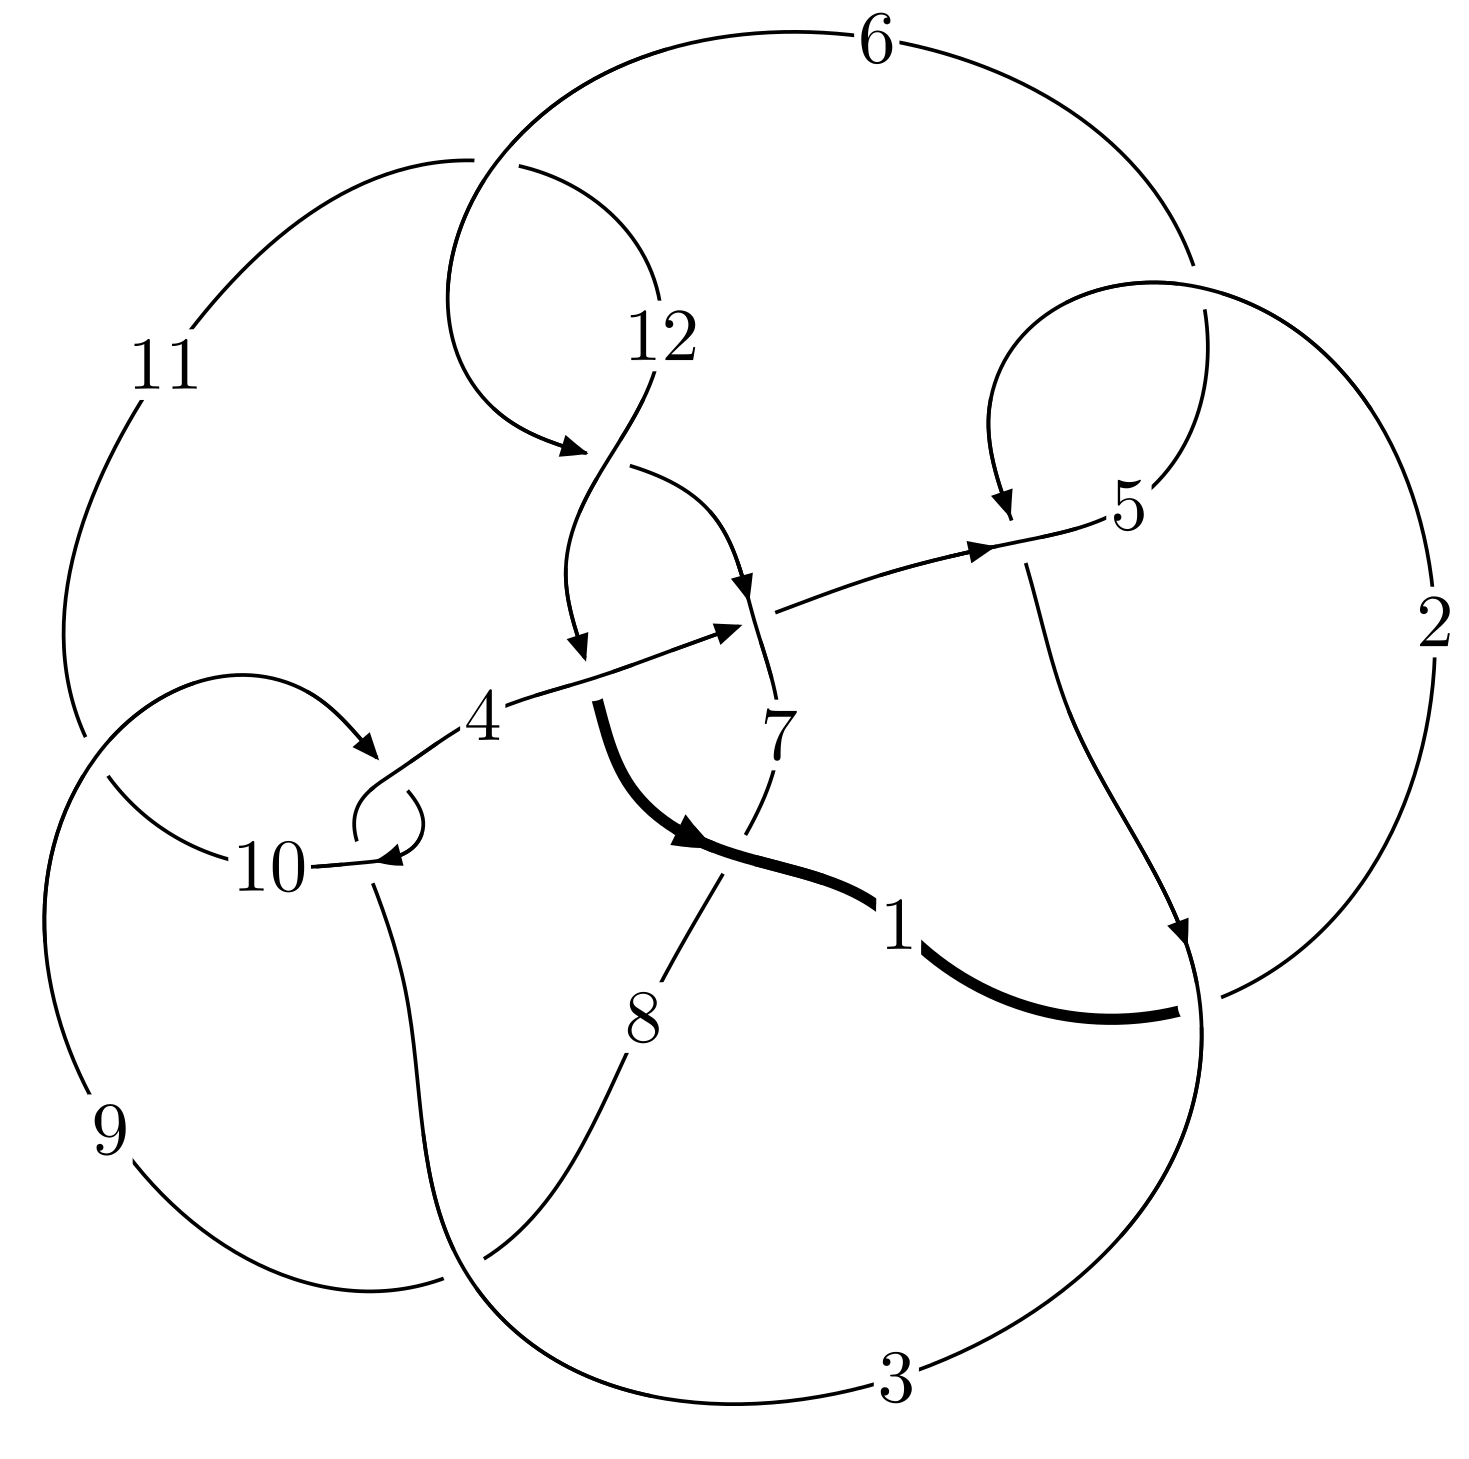
\includegraphics[width=112pt]{../../../GIT/diagram.site/Diagrams/png/2571_12n_0482.png}\\
\ \ \ A knot diagram\footnotemark}&
\allowdisplaybreaks
\textbf{Linearized knot diagam} \\
\cline{2-2}
 &
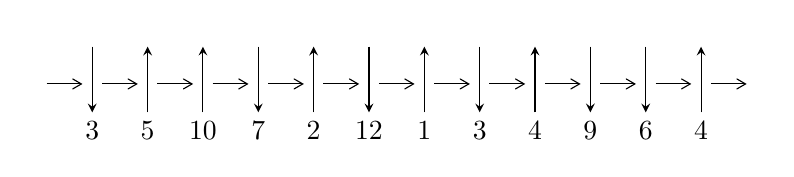
\begin{tikzpicture}[x=20pt, y=17pt]
	% nodes
	\node (C0) at (0, 0) {};
	\node (C1) at (1, 0) {};
	\node (C1U) at (1, +1) {};
	\node (C1D) at (1, -1) {3};

	\node (C2) at (2, 0) {};
	\node (C2U) at (2, +1) {};
	\node (C2D) at (2, -1) {5};

	\node (C3) at (3, 0) {};
	\node (C3U) at (3, +1) {};
	\node (C3D) at (3, -1) {10};

	\node (C4) at (4, 0) {};
	\node (C4U) at (4, +1) {};
	\node (C4D) at (4, -1) {7};

	\node (C5) at (5, 0) {};
	\node (C5U) at (5, +1) {};
	\node (C5D) at (5, -1) {2};

	\node (C6) at (6, 0) {};
	\node (C6U) at (6, +1) {};
	\node (C6D) at (6, -1) {12};

	\node (C7) at (7, 0) {};
	\node (C7U) at (7, +1) {};
	\node (C7D) at (7, -1) {1};

	\node (C8) at (8, 0) {};
	\node (C8U) at (8, +1) {};
	\node (C8D) at (8, -1) {3};

	\node (C9) at (9, 0) {};
	\node (C9U) at (9, +1) {};
	\node (C9D) at (9, -1) {4};

	\node (C10) at (10, 0) {};
	\node (C10U) at (10, +1) {};
	\node (C10D) at (10, -1) {9};

	\node (C11) at (11, 0) {};
	\node (C11U) at (11, +1) {};
	\node (C11D) at (11, -1) {6};

	\node (C12) at (12, 0) {};
	\node (C12U) at (12, +1) {};
	\node (C12D) at (12, -1) {4};
	\node (C13) at (13, 0) {};

	% arrows
	\draw[->,>={angle 60}]
	(C0) edge (C1) (C1) edge (C2) (C2) edge (C3) (C3) edge (C4) (C4) edge (C5) (C5) edge (C6) (C6) edge (C7) (C7) edge (C8) (C8) edge (C9) (C9) edge (C10) (C10) edge (C11) (C11) edge (C12) (C12) edge (C13) ;	\draw[->,>=stealth]
	(C1U) edge (C1D) (C2D) edge (C2U) (C3D) edge (C3U) (C4U) edge (C4D) (C5D) edge (C5U) (C6U) edge (C6D) (C7D) edge (C7U) (C8U) edge (C8D) (C9D) edge (C9U) (C10U) edge (C10D) (C11U) edge (C11D) (C12D) edge (C12U) ;
	\end{tikzpicture} \\
\hhline{~~} \\& 
\textbf{Solving Sequence} \\ \cline{2-2} 
 &
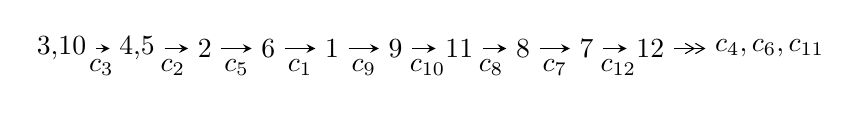
\begin{tikzpicture}[x=23pt, y=7pt]
	% node
	\node (A0) at (-1/8, 0) {3,10};
	\node (A1) at (17/16, 0) {4,5};
	\node (A2) at (17/8, 0) {2};
	\node (A3) at (25/8, 0) {6};
	\node (A4) at (33/8, 0) {1};
	\node (A5) at (41/8, 0) {9};
	\node (A6) at (49/8, 0) {11};
	\node (A7) at (57/8, 0) {8};
	\node (A8) at (65/8, 0) {7};
	\node (A9) at (73/8, 0) {12};
	\node (C1) at (1/2, -1) {$c_{3}$};
	\node (C2) at (13/8, -1) {$c_{2}$};
	\node (C3) at (21/8, -1) {$c_{5}$};
	\node (C4) at (29/8, -1) {$c_{1}$};
	\node (C5) at (37/8, -1) {$c_{9}$};
	\node (C6) at (45/8, -1) {$c_{10}$};
	\node (C7) at (53/8, -1) {$c_{8}$};
	\node (C8) at (61/8, -1) {$c_{7}$};
	\node (C9) at (69/8, -1) {$c_{12}$};
	\node (A10) at (11, 0) {$c_{4},c_{6},c_{11}$};

	% edge
	\draw[->,>=stealth]	
	(A0) edge (A1) (A1) edge (A2) (A2) edge (A3) (A3) edge (A4) (A4) edge (A5) (A5) edge (A6) (A6) edge (A7) (A7) edge (A8) (A8) edge (A9) ;
	\draw[->>,>={angle 60}]	
	(A9) edge (A10);
\end{tikzpicture} \\ 

\end{tabular} \\

\footnotetext{
The image of knot diagram is generated by the software ``\textbf{Draw programme}" developed by Andrew Bartholomew(\url{http://www.layer8.co.uk/maths/draw/index.htm\#Running-draw}), where we modified some parts for our purpose(\url{https://github.com/CATsTAILs/LinksPainter}).
}\phantom \\ \newline 
\centering \textbf{Ideals for irreducible components\footnotemark of $X_{\text{par}}$} 
 
\begin{align*}
I^u_{1}&=\langle 
b+u,\;135 u^{10}-671 u^9+\cdots+493 a+107,\\
\phantom{I^u_{1}}&\phantom{= \langle  }u^{11}-2 u^{10}+3 u^9-4 u^8+8 u^7-11 u^6+12 u^5-11 u^4+5 u^3-3 u^2-1\rangle \\
I^u_{2}&=\langle 
1.98818\times10^{32} u^{37}+5.18591\times10^{31} u^{36}+\cdots+3.87572\times10^{32} b-1.54819\times10^{32},\\
\phantom{I^u_{2}}&\phantom{= \langle  }4.74622\times10^{33} u^{37}+1.04073\times10^{33} u^{36}+\cdots+3.87572\times10^{32} a-3.08284\times10^{33},\;u^{38}+u^{37}+\cdots+11 u+1\rangle \\
I^u_{3}&=\langle 
b+u,\;-3 u^4+3 u^3-2 u^2+a+5 u-2,\;u^5- u^4+u^3-2 u^2+u-1\rangle \\
I^u_{4}&=\langle 
b+u,\;a+2 u+2,\;u^2+u+1\rangle \\
I^u_{5}&=\langle 
- u^{13}-2 u^{12}-3 u^{11}-8 u^{10}-7 u^9-16 u^8-10 u^7-21 u^6-13 u^5-18 u^4-9 u^3-11 u^2+b-3 u-2,\\
\phantom{I^u_{5}}&\phantom{= \langle  }3 u^{13}- u^{12}+10 u^{11}+19 u^9+2 u^8+22 u^7+8 u^6+19 u^5+5 u^4+12 u^3+3 u^2+a+2 u,\\
\phantom{I^u_{5}}&\phantom{= \langle  }u^{14}+4 u^{12}+u^{11}+9 u^{10}+3 u^9+13 u^8+6 u^7+14 u^6+6 u^5+11 u^4+4 u^3+5 u^2+u+1\rangle \\
\\
\end{align*}
\raggedright * 5 irreducible components of $\dim_{\mathbb{C}}=0$, with total 70 representations.\\
\footnotetext{All coefficients of polynomials are rational numbers. But the coefficients are sometimes approximated in decimal forms when there is not enough margin.}
\newpage
\renewcommand{\arraystretch}{1}
\centering \section*{I. $I^u_{1}= \langle b+u,\;135 u^{10}-671 u^9+\cdots+493 a+107,\;u^{11}-2 u^{10}+\cdots-3 u^2-1 \rangle$}
\flushleft \textbf{(i) Arc colorings}\\
\begin{tabular}{m{7pt} m{180pt} m{7pt} m{180pt} }
\flushright $a_{3}=$&$\begin{pmatrix}1\\0\end{pmatrix}$ \\
\flushright $a_{10}=$&$\begin{pmatrix}0\\u\end{pmatrix}$ \\
\flushright $a_{4}=$&$\begin{pmatrix}1\\- u^2\end{pmatrix}$ \\
\flushright $a_{5}=$&$\begin{pmatrix}-0.273834 u^{10}+1.36105 u^{9}+\cdots+3.25761 u-0.217039\\- u\end{pmatrix}$ \\
\flushright $a_{2}=$&$\begin{pmatrix}-0.813387 u^{10}+1.76876 u^{9}+\cdots+0.217039 u+1.27383\\u^2\end{pmatrix}$ \\
\flushright $a_{6}=$&$\begin{pmatrix}-0.415822 u^{10}+1.36308 u^{9}+\cdots+1.98377 u+0.596349\\- u^3- u\end{pmatrix}$ \\
\flushright $a_{1}=$&$\begin{pmatrix}-0.813387 u^{10}+1.76876 u^{9}+\cdots+0.217039 u+1.27383\\u^2\end{pmatrix}$ \\
\flushright $a_{9}=$&$\begin{pmatrix}- u\\u^3+u\end{pmatrix}$ \\
\flushright $a_{11}=$&$\begin{pmatrix}- u^3\\u^5+u^3+u\end{pmatrix}$ \\
\flushright $a_{8}=$&$\begin{pmatrix}u^3\\u^3+u\end{pmatrix}$ \\
\flushright $a_{7}=$&$\begin{pmatrix}0.0263692 u^{10}-0.271805 u^{9}+\cdots-3.30629 u+1.00609\\0.0953347 u^{10}-0.444219 u^{9}+\cdots+0.969574 u-0.131846\end{pmatrix}$ \\
\flushright $a_{12}=$&$\begin{pmatrix}-1.09533 u^{10}+2.44422 u^{9}+\cdots+1.03043 u+1.13185\\-0.150101 u^{10}+0.316430 u^{9}+\cdots+0.281947 u-0.111562\end{pmatrix}$\\&\end{tabular}
\flushleft \textbf{(ii) Obstruction class $= -1$}\\~\\
\flushleft \textbf{(iii) Cusp Shapes $= \frac{1818}{493} u^{10}-\frac{2167}{493} u^9+\frac{2637}{493} u^8-\frac{3733}{493} u^7+\frac{10857}{493} u^6-\frac{10419}{493} u^5+\frac{8712}{493} u^4-\frac{7389}{493} u^3+\frac{2214}{493} u^2-\frac{3255}{493} u-\frac{301}{493}$}\\~\\
\newpage\renewcommand{\arraystretch}{1}
\flushleft \textbf{(iv) u-Polynomials at the component}\newline \\
\begin{tabular}{m{50pt}|m{274pt}}
Crossings & \hspace{64pt}u-Polynomials at each crossing \\
\hline $$\begin{aligned}c_{1},c_{10}\end{aligned}$$&$\begin{aligned}
&u^{11}+2 u^{10}+\cdots-6 u-1
\end{aligned}$\\
\hline $$\begin{aligned}c_{2},c_{3},c_{5}\\c_{9}\end{aligned}$$&$\begin{aligned}
&u^{11}-2 u^{10}+3 u^9-4 u^8+8 u^7-11 u^6+12 u^5-11 u^4+5 u^3-3 u^2-1
\end{aligned}$\\
\hline $$\begin{aligned}c_{4},c_{6},c_{11}\end{aligned}$$&$\begin{aligned}
&u^{11}- u^{10}- u^9+u^8+5 u^7-3 u^6-4 u^5+u^4+3 u^3- u^2+3 u-1
\end{aligned}$\\
\hline $$\begin{aligned}c_{7}\end{aligned}$$&$\begin{aligned}
&u^{11}+u^{10}+\cdots-51 u-17
\end{aligned}$\\
\hline $$\begin{aligned}c_{8}\end{aligned}$$&$\begin{aligned}
&u^{11}-4 u^{10}+\cdots-16 u-1
\end{aligned}$\\
\hline $$\begin{aligned}c_{12}\end{aligned}$$&$\begin{aligned}
&u^{11}+8 u^{10}+\cdots-320 u-64
\end{aligned}$\\
\hline
\end{tabular}\\~\\
\newpage\renewcommand{\arraystretch}{1}
\flushleft \textbf{(v) Riley Polynomials at the component}\newline \\
\begin{tabular}{m{50pt}|m{274pt}}
Crossings & \hspace{64pt}Riley Polynomials at each crossing \\
\hline $$\begin{aligned}c_{1},c_{10}\end{aligned}$$&$\begin{aligned}
&y^{11}+14 y^{10}+\cdots-26 y-1
\end{aligned}$\\
\hline $$\begin{aligned}c_{2},c_{3},c_{5}\\c_{9}\end{aligned}$$&$\begin{aligned}
&y^{11}+2 y^{10}+\cdots-6 y-1
\end{aligned}$\\
\hline $$\begin{aligned}c_{4},c_{6},c_{11}\end{aligned}$$&$\begin{aligned}
&y^{11}-3 y^{10}+\cdots+7 y-1
\end{aligned}$\\
\hline $$\begin{aligned}c_{7}\end{aligned}$$&$\begin{aligned}
&y^{11}-15 y^{10}+\cdots-425 y-289
\end{aligned}$\\
\hline $$\begin{aligned}c_{8}\end{aligned}$$&$\begin{aligned}
&y^{11}+20 y^{10}+\cdots+92 y-1
\end{aligned}$\\
\hline $$\begin{aligned}c_{12}\end{aligned}$$&$\begin{aligned}
&y^{11}-22 y^{10}+\cdots-10240 y-4096
\end{aligned}$\\
\hline
\end{tabular}\\~\\
\newpage\flushleft \textbf{(vi) Complex Volumes and Cusp Shapes}
$$\begin{array}{c|c|c}  
\text{Solutions to }I^u_{1}& \I (\text{vol} + \sqrt{-1}CS) & \text{Cusp shape}\\
 \hline 
\begin{aligned}
u &= \phantom{-}0.069055 + 1.000350 I \\
a &= -0.981312 - 0.304041 I \\
b &= -0.069055 - 1.000350 I\end{aligned}
 & -5.87879 + 3.62795 I & -10.28819 - 4.50965 I \\ \hline\begin{aligned}
u &= \phantom{-}0.069055 - 1.000350 I \\
a &= -0.981312 + 0.304041 I \\
b &= -0.069055 + 1.000350 I\end{aligned}
 & -5.87879 - 3.62795 I & -10.28819 + 4.50965 I \\ \hline\begin{aligned}
u &= \phantom{-}0.457197 + 0.753480 I \\
a &= \phantom{-}0.883878 - 0.436496 I \\
b &= -0.457197 - 0.753480 I\end{aligned}
 & \phantom{-}0.73694 + 2.00002 I & \phantom{-}2.64478 - 3.99897 I \\ \hline\begin{aligned}
u &= \phantom{-}0.457197 - 0.753480 I \\
a &= \phantom{-}0.883878 + 0.436496 I \\
b &= -0.457197 + 0.753480 I\end{aligned}
 & \phantom{-}0.73694 - 2.00002 I & \phantom{-}2.64478 + 3.99897 I \\ \hline\begin{aligned}
u &= \phantom{-}1.21408\phantom{ +0.000000I} \\
a &= \phantom{-}0.899878\phantom{ +0.000000I} \\
b &= -1.21408\phantom{ +0.000000I}\end{aligned}
 & \phantom{-}2.41788\phantom{ +0.000000I} & \phantom{-}20.6200\phantom{ +0.000000I} \\ \hline\begin{aligned}
u &= \phantom{-}1.06044 + 0.99031 I \\
a &= \phantom{-}1.37322 - 0.35892 I \\
b &= -1.06044 - 0.99031 I\end{aligned}
 & \phantom{-}10.12310 + 0.00215 I & \phantom{-}1.32048 + 0.53124 I \\ \hline\begin{aligned}
u &= \phantom{-}1.06044 - 0.99031 I \\
a &= \phantom{-}1.37322 + 0.35892 I \\
b &= -1.06044 + 0.99031 I\end{aligned}
 & \phantom{-}10.12310 - 0.00215 I & \phantom{-}1.32048 - 0.53124 I \\ \hline\begin{aligned}
u &= -0.92863 + 1.13891 I \\
a &= -1.51448 - 0.57303 I \\
b &= \phantom{-}0.92863 - 1.13891 I\end{aligned}
 & \phantom{-}8.9020 - 15.0293 I & -0.32227 + 7.97448 I \\ \hline\begin{aligned}
u &= -0.92863 - 1.13891 I \\
a &= -1.51448 + 0.57303 I \\
b &= \phantom{-}0.92863 + 1.13891 I\end{aligned}
 & \phantom{-}8.9020 + 15.0293 I & -0.32227 - 7.97448 I \\ \hline\begin{aligned}
u &= -0.265103 + 0.402117 I \\
a &= \phantom{-}1.28876 + 2.59793 I \\
b &= \phantom{-}0.265103 - 0.402117 I\end{aligned}
 & -1.93271 + 1.18056 I & -1.16495 - 2.63475 I\\
 \hline 
 \end{array}$$\newpage$$\begin{array}{c|c|c}  
\text{Solutions to }I^u_{1}& \I (\text{vol} + \sqrt{-1}CS) & \text{Cusp shape}\\
 \hline 
\begin{aligned}
u &= -0.265103 - 0.402117 I \\
a &= \phantom{-}1.28876 - 2.59793 I \\
b &= \phantom{-}0.265103 + 0.402117 I\end{aligned}
 & -1.93271 - 1.18056 I & -1.16495 + 2.63475 I\\
 \hline 
 \end{array}$$\newpage\newpage\renewcommand{\arraystretch}{1}
\centering \section*{II. $I^u_{2}= \langle 1.99\times10^{32} u^{37}+5.19\times10^{31} u^{36}+\cdots+3.88\times10^{32} b-1.55\times10^{32},\;4.75\times10^{33} u^{37}+1.04\times10^{33} u^{36}+\cdots+3.88\times10^{32} a-3.08\times10^{33},\;u^{38}+u^{37}+\cdots+11 u+1 \rangle$}
\flushleft \textbf{(i) Arc colorings}\\
\begin{tabular}{m{7pt} m{180pt} m{7pt} m{180pt} }
\flushright $a_{3}=$&$\begin{pmatrix}1\\0\end{pmatrix}$ \\
\flushright $a_{10}=$&$\begin{pmatrix}0\\u\end{pmatrix}$ \\
\flushright $a_{4}=$&$\begin{pmatrix}1\\- u^2\end{pmatrix}$ \\
\flushright $a_{5}=$&$\begin{pmatrix}-12.2460 u^{37}-2.68526 u^{36}+\cdots+1.99894 u+7.95423\\-0.512982 u^{37}-0.133805 u^{36}+\cdots+0.536992 u+0.399459\end{pmatrix}$ \\
\flushright $a_{2}=$&$\begin{pmatrix}7.74425 u^{37}+4.31734 u^{36}+\cdots+215.566 u+26.2164\\0.565194 u^{37}+2.66371 u^{36}+\cdots+55.8911 u+6.22476\end{pmatrix}$ \\
\flushright $a_{6}=$&$\begin{pmatrix}-11.1078 u^{37}-6.54371 u^{36}+\cdots-143.314 u-12.5852\\3.29534 u^{37}+2.38055 u^{36}+\cdots+112.115 u+12.6582\end{pmatrix}$ \\
\flushright $a_{1}=$&$\begin{pmatrix}8.30944 u^{37}+6.98105 u^{36}+\cdots+271.458 u+32.4411\\0.565194 u^{37}+2.66371 u^{36}+\cdots+55.8911 u+6.22476\end{pmatrix}$ \\
\flushright $a_{9}=$&$\begin{pmatrix}- u\\u^3+u\end{pmatrix}$ \\
\flushright $a_{11}=$&$\begin{pmatrix}- u^3\\u^5+u^3+u\end{pmatrix}$ \\
\flushright $a_{8}=$&$\begin{pmatrix}u^3\\u^3+u\end{pmatrix}$ \\
\flushright $a_{7}=$&$\begin{pmatrix}2.38323 u^{37}+1.44709 u^{36}+\cdots+51.2510 u+3.28992\\1.45749 u^{37}+1.85739 u^{36}+\cdots+1.74398 u-1.81804\end{pmatrix}$ \\
\flushright $a_{12}=$&$\begin{pmatrix}7.40661 u^{37}+4.29257 u^{36}+\cdots+209.264 u+24.8880\\-1.35180 u^{37}+1.74929 u^{36}+\cdots+35.3462 u+4.43912\end{pmatrix}$\\&\end{tabular}
\flushleft \textbf{(ii) Obstruction class $= -1$}\\~\\
\flushleft \textbf{(iii) Cusp Shapes $= 25.3622 u^{37}+20.1574 u^{36}+\cdots+887.101 u+105.896$}\\~\\
\newpage\renewcommand{\arraystretch}{1}
\flushleft \textbf{(iv) u-Polynomials at the component}\newline \\
\begin{tabular}{m{50pt}|m{274pt}}
Crossings & \hspace{64pt}u-Polynomials at each crossing \\
\hline $$\begin{aligned}c_{1},c_{10}\end{aligned}$$&$\begin{aligned}
&u^{38}+7 u^{37}+\cdots-3 u+1
\end{aligned}$\\
\hline $$\begin{aligned}c_{2},c_{3},c_{5}\\c_{9}\end{aligned}$$&$\begin{aligned}
&u^{38}+u^{37}+\cdots+11 u+1
\end{aligned}$\\
\hline $$\begin{aligned}c_{4},c_{6},c_{11}\end{aligned}$$&$\begin{aligned}
&u^{38}+u^{37}+\cdots-13 u+1
\end{aligned}$\\
\hline $$\begin{aligned}c_{7}\end{aligned}$$&$\begin{aligned}
&u^{38}+6 u^{37}+\cdots+279558 u+34943
\end{aligned}$\\
\hline $$\begin{aligned}c_{8}\end{aligned}$$&$\begin{aligned}
&u^{38}+2 u^{37}+\cdots+31225 u+84625
\end{aligned}$\\
\hline $$\begin{aligned}c_{12}\end{aligned}$$&$\begin{aligned}
&(u^{19}-4 u^{18}+\cdots+182 u-103)^{2}
\end{aligned}$\\
\hline
\end{tabular}\\~\\
\newpage\renewcommand{\arraystretch}{1}
\flushleft \textbf{(v) Riley Polynomials at the component}\newline \\
\begin{tabular}{m{50pt}|m{274pt}}
Crossings & \hspace{64pt}Riley Polynomials at each crossing \\
\hline $$\begin{aligned}c_{1},c_{10}\end{aligned}$$&$\begin{aligned}
&y^{38}+47 y^{37}+\cdots+41 y+1
\end{aligned}$\\
\hline $$\begin{aligned}c_{2},c_{3},c_{5}\\c_{9}\end{aligned}$$&$\begin{aligned}
&y^{38}+7 y^{37}+\cdots-3 y+1
\end{aligned}$\\
\hline $$\begin{aligned}c_{4},c_{6},c_{11}\end{aligned}$$&$\begin{aligned}
&y^{38}-7 y^{37}+\cdots-27 y+1
\end{aligned}$\\
\hline $$\begin{aligned}c_{7}\end{aligned}$$&$\begin{aligned}
&y^{38}-54 y^{37}+\cdots+19424324302 y+1221013249
\end{aligned}$\\
\hline $$\begin{aligned}c_{8}\end{aligned}$$&$\begin{aligned}
&y^{38}+90 y^{37}+\cdots+115039950625 y+7161390625
\end{aligned}$\\
\hline $$\begin{aligned}c_{12}\end{aligned}$$&$\begin{aligned}
&(y^{19}-18 y^{18}+\cdots-49070 y-10609)^{2}
\end{aligned}$\\
\hline
\end{tabular}\\~\\
\newpage\flushleft \textbf{(vi) Complex Volumes and Cusp Shapes}
$$\begin{array}{c|c|c}  
\text{Solutions to }I^u_{2}& \I (\text{vol} + \sqrt{-1}CS) & \text{Cusp shape}\\
 \hline 
\begin{aligned}
u &= \phantom{-}1.004590 + 0.172131 I \\
a &= \phantom{-}0.883738 - 0.151424 I \\
b &= -1.004590 + 0.172131 I\end{aligned}
 & \phantom{-}2.25367\phantom{ +0.000000I} & \phantom{-}8.32597 + 0. I\phantom{ +0.000000I} \\ \hline\begin{aligned}
u &= \phantom{-}1.004590 - 0.172131 I \\
a &= \phantom{-}0.883738 + 0.151424 I \\
b &= -1.004590 - 0.172131 I\end{aligned}
 & \phantom{-}2.25367\phantom{ +0.000000I} & \phantom{-}8.32597 + 0. I\phantom{ +0.000000I} \\ \hline\begin{aligned}
u &= -0.769998 + 0.586991 I \\
a &= \phantom{-}1.117170 + 0.263942 I \\
b &= -0.49939 + 1.38926 I\end{aligned}
 & -1.95090 - 5.96839 I & \phantom{-}0.62541 + 10.55313 I \\ \hline\begin{aligned}
u &= -0.769998 - 0.586991 I \\
a &= \phantom{-}1.117170 - 0.263942 I \\
b &= -0.49939 - 1.38926 I\end{aligned}
 & -1.95090 + 5.96839 I & \phantom{-}0.62541 - 10.55313 I \\ \hline\begin{aligned}
u &= -0.250368 + 0.928587 I \\
a &= \phantom{-}0.922332 + 0.890681 I \\
b &= \phantom{-}0.516346 + 1.055000 I\end{aligned}
 & -3.76429 + 1.96233 I & -6.97090 - 0.90766 I \\ \hline\begin{aligned}
u &= -0.250368 - 0.928587 I \\
a &= \phantom{-}0.922332 - 0.890681 I \\
b &= \phantom{-}0.516346 - 1.055000 I\end{aligned}
 & -3.76429 - 1.96233 I & -6.97090 + 0.90766 I \\ \hline\begin{aligned}
u &= \phantom{-}0.685299 + 0.877713 I \\
a &= \phantom{-}0.431131 + 0.017894 I \\
b &= \phantom{-}0.221102 - 0.581236 I\end{aligned}
 & \phantom{-}0.80155 + 2.69495 I & \phantom{-}4.30397 - 0.26494 I \\ \hline\begin{aligned}
u &= \phantom{-}0.685299 - 0.877713 I \\
a &= \phantom{-}0.431131 - 0.017894 I \\
b &= \phantom{-}0.221102 + 0.581236 I\end{aligned}
 & \phantom{-}0.80155 - 2.69495 I & \phantom{-}4.30397 + 0.26494 I \\ \hline\begin{aligned}
u &= -0.151590 + 0.840331 I \\
a &= \phantom{-}1.15667 + 1.14014 I \\
b &= \phantom{-}0.319310 + 0.249382 I\end{aligned}
 & -1.87491 + 1.48071 I & -3.81413 - 3.72384 I \\ \hline\begin{aligned}
u &= -0.151590 - 0.840331 I \\
a &= \phantom{-}1.15667 - 1.14014 I \\
b &= \phantom{-}0.319310 - 0.249382 I\end{aligned}
 & -1.87491 - 1.48071 I & -3.81413 + 3.72384 I\\
 \hline 
 \end{array}$$\newpage$$\begin{array}{c|c|c}  
\text{Solutions to }I^u_{2}& \I (\text{vol} + \sqrt{-1}CS) & \text{Cusp shape}\\
 \hline 
\begin{aligned}
u &= -0.479231 + 1.064790 I \\
a &= -1.79535 - 0.55808 I \\
b &= \phantom{-}0.350575 - 0.499346 I\end{aligned}
 & -3.82831 - 4.84634 I & -7.70612 + 6.88664 I \\ \hline\begin{aligned}
u &= -0.479231 - 1.064790 I \\
a &= -1.79535 + 0.55808 I \\
b &= \phantom{-}0.350575 + 0.499346 I\end{aligned}
 & -3.82831 + 4.84634 I & -7.70612 - 6.88664 I \\ \hline\begin{aligned}
u &= \phantom{-}0.908346 + 0.735932 I \\
a &= -0.339798 - 0.249688 I \\
b &= \phantom{-}0.400909 + 0.103737 I\end{aligned}
 & \phantom{-}1.01937 + 3.04219 I & \phantom{-}4.58994 - 7.02078 I \\ \hline\begin{aligned}
u &= \phantom{-}0.908346 - 0.735932 I \\
a &= -0.339798 + 0.249688 I \\
b &= \phantom{-}0.400909 - 0.103737 I\end{aligned}
 & \phantom{-}1.01937 - 3.04219 I & \phantom{-}4.58994 + 7.02078 I \\ \hline\begin{aligned}
u &= -0.516346 + 1.055000 I \\
a &= -0.088440 + 1.046130 I \\
b &= \phantom{-}0.250368 + 0.928587 I\end{aligned}
 & -3.76429 - 1.96233 I & -6.97090 + 0.90766 I \\ \hline\begin{aligned}
u &= -0.516346 - 1.055000 I \\
a &= -0.088440 - 1.046130 I \\
b &= \phantom{-}0.250368 - 0.928587 I\end{aligned}
 & -3.76429 + 1.96233 I & -6.97090 - 0.90766 I \\ \hline\begin{aligned}
u &= -1.044560 + 0.842557 I \\
a &= -0.811923 - 0.654907 I \\
b &= \phantom{-}1.044560 + 0.842557 I\end{aligned}
 & \phantom{-}10.6548\phantom{ +0.000000I} & \phantom{-0.000000 } 0 \\ \hline\begin{aligned}
u &= -1.044560 - 0.842557 I \\
a &= -0.811923 + 0.654907 I \\
b &= \phantom{-}1.044560 - 0.842557 I\end{aligned}
 & \phantom{-}10.6548\phantom{ +0.000000I} & \phantom{-0.000000 } 0 \\ \hline\begin{aligned}
u &= \phantom{-}0.976290 + 0.949251 I \\
a &= -1.63572 + 0.33244 I \\
b &= \phantom{-}0.887628 + 1.095510 I\end{aligned}
 & \phantom{-}9.80034 + 7.08036 I & \phantom{-0.000000 } 0. - 4.76593 I \\ \hline\begin{aligned}
u &= \phantom{-}0.976290 - 0.949251 I \\
a &= -1.63572 - 0.33244 I \\
b &= \phantom{-}0.887628 - 1.095510 I\end{aligned}
 & \phantom{-}9.80034 - 7.08036 I & \phantom{-0.000000 -}0. + 4.76593 I\\
 \hline 
 \end{array}$$\newpage$$\begin{array}{c|c|c}  
\text{Solutions to }I^u_{2}& \I (\text{vol} + \sqrt{-1}CS) & \text{Cusp shape}\\
 \hline 
\begin{aligned}
u &= -0.221102 + 0.581236 I \\
a &= \phantom{-}0.427232 - 0.643816 I \\
b &= -0.685299 - 0.877713 I\end{aligned}
 & \phantom{-}0.80155 + 2.69495 I & \phantom{-}4.30397 - 0.26494 I \\ \hline\begin{aligned}
u &= -0.221102 - 0.581236 I \\
a &= \phantom{-}0.427232 + 0.643816 I \\
b &= -0.685299 + 0.877713 I\end{aligned}
 & \phantom{-}0.80155 - 2.69495 I & \phantom{-}4.30397 + 0.26494 I \\ \hline\begin{aligned}
u &= \phantom{-}0.950416 + 1.005200 I \\
a &= \phantom{-}0.568027 - 0.600769 I \\
b &= -0.950416 + 1.005200 I\end{aligned}
 & \phantom{-}9.62378\phantom{ +0.000000I} & \phantom{-0.000000 } 0 \\ \hline\begin{aligned}
u &= \phantom{-}0.950416 - 1.005200 I \\
a &= \phantom{-}0.568027 + 0.600769 I \\
b &= -0.950416 - 1.005200 I\end{aligned}
 & \phantom{-}9.62378\phantom{ +0.000000I} & \phantom{-0.000000 } 0 \\ \hline\begin{aligned}
u &= -0.350575 + 0.499346 I \\
a &= -3.57554 - 0.40279 I \\
b &= \phantom{-}0.479231 - 1.064790 I\end{aligned}
 & -3.82831 - 4.84634 I & -7.70612 + 6.88664 I \\ \hline\begin{aligned}
u &= -0.350575 - 0.499346 I \\
a &= -3.57554 + 0.40279 I \\
b &= \phantom{-}0.479231 + 1.064790 I\end{aligned}
 & -3.82831 + 4.84634 I & -7.70612 - 6.88664 I \\ \hline\begin{aligned}
u &= -0.887628 + 1.095510 I \\
a &= \phantom{-}1.53068 + 0.50554 I \\
b &= -0.976290 + 0.949251 I\end{aligned}
 & \phantom{-}9.80034 - 7.08036 I & \phantom{-0.000000 } 0 \\ \hline\begin{aligned}
u &= -0.887628 - 1.095510 I \\
a &= \phantom{-}1.53068 - 0.50554 I \\
b &= -0.976290 - 0.949251 I\end{aligned}
 & \phantom{-}9.80034 + 7.08036 I & \phantom{-0.000000 } 0 \\ \hline\begin{aligned}
u &= -1.14162 + 0.84482 I \\
a &= \phantom{-}0.714096 + 0.478108 I \\
b &= -1.00890 - 1.04517 I\end{aligned}
 & \phantom{-}9.91517 + 7.54398 I & \phantom{-0.000000 } 0 \\ \hline\begin{aligned}
u &= -1.14162 - 0.84482 I \\
a &= \phantom{-}0.714096 - 0.478108 I \\
b &= -1.00890 + 1.04517 I\end{aligned}
 & \phantom{-}9.91517 - 7.54398 I & \phantom{-0.000000 } 0\\
 \hline 
 \end{array}$$\newpage$$\begin{array}{c|c|c}  
\text{Solutions to }I^u_{2}& \I (\text{vol} + \sqrt{-1}CS) & \text{Cusp shape}\\
 \hline 
\begin{aligned}
u &= \phantom{-}1.00890 + 1.04517 I \\
a &= -0.554397 + 0.631289 I \\
b &= \phantom{-}1.14162 - 0.84482 I\end{aligned}
 & \phantom{-}9.91517 + 7.54398 I & \phantom{-0.000000 } 0 \\ \hline\begin{aligned}
u &= \phantom{-}1.00890 - 1.04517 I \\
a &= -0.554397 - 0.631289 I \\
b &= \phantom{-}1.14162 + 0.84482 I\end{aligned}
 & \phantom{-}9.91517 - 7.54398 I & \phantom{-0.000000 } 0 \\ \hline\begin{aligned}
u &= \phantom{-}0.49939 + 1.38926 I \\
a &= -0.521072 + 0.543402 I \\
b &= \phantom{-}0.769998 + 0.586991 I\end{aligned}
 & -1.95090 + 5.96839 I & \phantom{-0.000000 } 0 \\ \hline\begin{aligned}
u &= \phantom{-}0.49939 - 1.38926 I \\
a &= -0.521072 - 0.543402 I \\
b &= \phantom{-}0.769998 - 0.586991 I\end{aligned}
 & -1.95090 - 5.96839 I & \phantom{-0.000000 } 0 \\ \hline\begin{aligned}
u &= -0.400909 + 0.103737 I \\
a &= \phantom{-}0.580462 - 1.039280 I \\
b &= -0.908346 + 0.735932 I\end{aligned}
 & \phantom{-}1.01937 - 3.04219 I & \phantom{-}4.58994 + 7.02078 I \\ \hline\begin{aligned}
u &= -0.400909 - 0.103737 I \\
a &= \phantom{-}0.580462 + 1.039280 I \\
b &= -0.908346 - 0.735932 I\end{aligned}
 & \phantom{-}1.01937 + 3.04219 I & \phantom{-}4.58994 - 7.02078 I \\ \hline\begin{aligned}
u &= -0.319310 + 0.249382 I \\
a &= \phantom{-}0.99071 + 3.27648 I \\
b &= \phantom{-}0.151590 + 0.840331 I\end{aligned}
 & -1.87491 - 1.48071 I & -3.81413 + 3.72384 I \\ \hline\begin{aligned}
u &= -0.319310 - 0.249382 I \\
a &= \phantom{-}0.99071 - 3.27648 I \\
b &= \phantom{-}0.151590 - 0.840331 I\end{aligned}
 & -1.87491 + 1.48071 I & -3.81413 - 3.72384 I\\
 \hline 
 \end{array}$$\newpage\newpage\renewcommand{\arraystretch}{1}
\centering \section*{III. $I^u_{3}= \langle b+u,\;-3 u^4+3 u^3-2 u^2+a+5 u-2,\;u^5- u^4+u^3-2 u^2+u-1 \rangle$}
\flushleft \textbf{(i) Arc colorings}\\
\begin{tabular}{m{7pt} m{180pt} m{7pt} m{180pt} }
\flushright $a_{3}=$&$\begin{pmatrix}1\\0\end{pmatrix}$ \\
\flushright $a_{10}=$&$\begin{pmatrix}0\\u\end{pmatrix}$ \\
\flushright $a_{4}=$&$\begin{pmatrix}1\\- u^2\end{pmatrix}$ \\
\flushright $a_{5}=$&$\begin{pmatrix}3 u^4-3 u^3+2 u^2-5 u+2\\- u\end{pmatrix}$ \\
\flushright $a_{2}=$&$\begin{pmatrix}u^3- u^2+u-2\\u^2\end{pmatrix}$ \\
\flushright $a_{6}=$&$\begin{pmatrix}2 u^4-2 u^3+u^2-3 u+2\\- u^3- u\end{pmatrix}$ \\
\flushright $a_{1}=$&$\begin{pmatrix}u^3+u-2\\u^2\end{pmatrix}$ \\
\flushright $a_{9}=$&$\begin{pmatrix}- u\\u^3+u\end{pmatrix}$ \\
\flushright $a_{11}=$&$\begin{pmatrix}- u^3\\u^4+2 u^2+1\end{pmatrix}$ \\
\flushright $a_{8}=$&$\begin{pmatrix}u^3\\u^3+u\end{pmatrix}$ \\
\flushright $a_{7}=$&$\begin{pmatrix}u^4+u^3- u^2-2 u-1\\u^3- u^2+u-1\end{pmatrix}$ \\
\flushright $a_{12}=$&$\begin{pmatrix}- u^4+u^3- u^2+2 u-3\\u^4+3 u^2+1\end{pmatrix}$\\&\end{tabular}
\flushleft \textbf{(ii) Obstruction class $= 1$}\\~\\
\flushleft \textbf{(iii) Cusp Shapes $= u^4-2 u^3-7 u^2- u-12$}\\~\\
\newpage\renewcommand{\arraystretch}{1}
\flushleft \textbf{(iv) u-Polynomials at the component}\newline \\
\begin{tabular}{m{50pt}|m{274pt}}
Crossings & \hspace{64pt}u-Polynomials at each crossing \\
\hline $$\begin{aligned}c_{1}\end{aligned}$$&$\begin{aligned}
&u^5- u^4- u^3+4 u^2-3 u+1
\end{aligned}$\\
\hline $$\begin{aligned}c_{2},c_{9}\end{aligned}$$&$\begin{aligned}
&u^5+u^4+u^3+2 u^2+u+1
\end{aligned}$\\
\hline $$\begin{aligned}c_{3},c_{5}\end{aligned}$$&$\begin{aligned}
&u^5- u^4+u^3-2 u^2+u-1
\end{aligned}$\\
\hline $$\begin{aligned}c_{4},c_{6}\end{aligned}$$&$\begin{aligned}
&u^5-2 u^3+u^2+2 u-1
\end{aligned}$\\
\hline $$\begin{aligned}c_{7}\end{aligned}$$&$\begin{aligned}
&u^5+2 u^4+2 u^3+3 u^2+2 u+1
\end{aligned}$\\
\hline $$\begin{aligned}c_{8}\end{aligned}$$&$\begin{aligned}
&u^5+5 u^4+6 u^3+3 u^2+u+1
\end{aligned}$\\
\hline $$\begin{aligned}c_{10}\end{aligned}$$&$\begin{aligned}
&u^5+u^4- u^3-4 u^2-3 u-1
\end{aligned}$\\
\hline $$\begin{aligned}c_{11}\end{aligned}$$&$\begin{aligned}
&u^5-2 u^3- u^2+2 u+1
\end{aligned}$\\
\hline $$\begin{aligned}c_{12}\end{aligned}$$&$\begin{aligned}
&u^5+6 u^4+9 u^3+8 u^2+4 u+1
\end{aligned}$\\
\hline
\end{tabular}\\~\\
\newpage\renewcommand{\arraystretch}{1}
\flushleft \textbf{(v) Riley Polynomials at the component}\newline \\
\begin{tabular}{m{50pt}|m{274pt}}
Crossings & \hspace{64pt}Riley Polynomials at each crossing \\
\hline $$\begin{aligned}c_{1},c_{10}\end{aligned}$$&$\begin{aligned}
&y^5-3 y^4+3 y^3-8 y^2+y-1
\end{aligned}$\\
\hline $$\begin{aligned}c_{2},c_{3},c_{5}\\c_{9}\end{aligned}$$&$\begin{aligned}
&y^5+y^4- y^3-4 y^2-3 y-1
\end{aligned}$\\
\hline $$\begin{aligned}c_{4},c_{6},c_{11}\end{aligned}$$&$\begin{aligned}
&y^5-4 y^4+8 y^3-9 y^2+6 y-1
\end{aligned}$\\
\hline $$\begin{aligned}c_{7}\end{aligned}$$&$\begin{aligned}
&y^5-4 y^3-5 y^2-2 y-1
\end{aligned}$\\
\hline $$\begin{aligned}c_{8}\end{aligned}$$&$\begin{aligned}
&y^5-13 y^4+8 y^3-7 y^2-5 y-1
\end{aligned}$\\
\hline $$\begin{aligned}c_{12}\end{aligned}$$&$\begin{aligned}
&y^5-18 y^4-7 y^3-4 y^2-1
\end{aligned}$\\
\hline
\end{tabular}\\~\\
\newpage\flushleft \textbf{(vi) Complex Volumes and Cusp Shapes}
$$\begin{array}{c|c|c}  
\text{Solutions to }I^u_{3}& \I (\text{vol} + \sqrt{-1}CS) & \text{Cusp shape}\\
 \hline 
\begin{aligned}
u &= -0.428550 + 1.039280 I \\
a &= -1.54944 - 0.53709 I \\
b &= \phantom{-}0.428550 - 1.039280 I\end{aligned}
 & -5.20316 - 6.77491 I & -7.90607 + 7.89291 I \\ \hline\begin{aligned}
u &= -0.428550 - 1.039280 I \\
a &= -1.54944 + 0.53709 I \\
b &= \phantom{-}0.428550 + 1.039280 I\end{aligned}
 & -5.20316 + 6.77491 I & -7.90607 - 7.89291 I \\ \hline\begin{aligned}
u &= \phantom{-}0.276511 + 0.728237 I \\
a &= \phantom{-}1.09747 - 3.27495 I \\
b &= -0.276511 - 0.728237 I\end{aligned}
 & -2.50012 - 0.60716 I & -8.21805 - 3.47460 I \\ \hline\begin{aligned}
u &= \phantom{-}0.276511 - 0.728237 I \\
a &= \phantom{-}1.09747 + 3.27495 I \\
b &= -0.276511 + 0.728237 I\end{aligned}
 & -2.50012 + 0.60716 I & -8.21805 + 3.47460 I \\ \hline\begin{aligned}
u &= \phantom{-}1.30408\phantom{ +0.000000I} \\
a &= \phantom{-}0.903937\phantom{ +0.000000I} \\
b &= -1.30408\phantom{ +0.000000I}\end{aligned}
 & \phantom{-}2.24708\phantom{ +0.000000I} & -26.7520\phantom{ +0.000000I}\\
 \hline 
 \end{array}$$\newpage\newpage\renewcommand{\arraystretch}{1}
\centering \section*{IV. $I^u_{4}= \langle b+u,\;a+2 u+2,\;u^2+u+1 \rangle$}
\flushleft \textbf{(i) Arc colorings}\\
\begin{tabular}{m{7pt} m{180pt} m{7pt} m{180pt} }
\flushright $a_{3}=$&$\begin{pmatrix}1\\0\end{pmatrix}$ \\
\flushright $a_{10}=$&$\begin{pmatrix}0\\u\end{pmatrix}$ \\
\flushright $a_{4}=$&$\begin{pmatrix}1\\u+1\end{pmatrix}$ \\
\flushright $a_{5}=$&$\begin{pmatrix}-2 u-2\\- u\end{pmatrix}$ \\
\flushright $a_{2}=$&$\begin{pmatrix}-1\\- u-1\end{pmatrix}$ \\
\flushright $a_{6}=$&$\begin{pmatrix}- u-2\\- u-1\end{pmatrix}$ \\
\flushright $a_{1}=$&$\begin{pmatrix}- u-2\\- u-1\end{pmatrix}$ \\
\flushright $a_{9}=$&$\begin{pmatrix}- u\\u+1\end{pmatrix}$ \\
\flushright $a_{11}=$&$\begin{pmatrix}-1\\0\end{pmatrix}$ \\
\flushright $a_{8}=$&$\begin{pmatrix}1\\u+1\end{pmatrix}$ \\
\flushright $a_{7}=$&$\begin{pmatrix}- u+2\\u+2\end{pmatrix}$ \\
\flushright $a_{12}=$&$\begin{pmatrix}-2 u-2\\- u\end{pmatrix}$\\&\end{tabular}
\flushleft \textbf{(ii) Obstruction class $= -1$}\\~\\
\flushleft \textbf{(iii) Cusp Shapes $= 12 u+6$}\\~\\
\newpage\renewcommand{\arraystretch}{1}
\flushleft \textbf{(iv) u-Polynomials at the component}\newline \\
\begin{tabular}{m{50pt}|m{274pt}}
Crossings & \hspace{64pt}u-Polynomials at each crossing \\
\hline $$\begin{aligned}c_{1},c_{2},c_{3}\\c_{4},c_{5},c_{6}\\c_{9},c_{10},c_{11}\\c_{12}\end{aligned}$$&$\begin{aligned}
&u^2+u+1
\end{aligned}$\\
\hline $$\begin{aligned}c_{7},c_{8}\end{aligned}$$&$\begin{aligned}
&u^2- u+1
\end{aligned}$\\
\hline
\end{tabular}\\~\\
\newpage\renewcommand{\arraystretch}{1}
\flushleft \textbf{(v) Riley Polynomials at the component}\newline \\
\begin{tabular}{m{50pt}|m{274pt}}
Crossings & \hspace{64pt}Riley Polynomials at each crossing \\
\hline $$\begin{aligned}c_{1},c_{2},c_{3}\\c_{4},c_{5},c_{6}\\c_{7},c_{8},c_{9}\\c_{10},c_{11},c_{12}\end{aligned}$$&$\begin{aligned}
&y^2+y+1
\end{aligned}$\\
\hline
\end{tabular}\\~\\
\newpage\flushleft \textbf{(vi) Complex Volumes and Cusp Shapes}
$$\begin{array}{c|c|c}  
\text{Solutions to }I^u_{4}& \I (\text{vol} + \sqrt{-1}CS) & \text{Cusp shape}\\
 \hline 
\begin{aligned}
u &= -0.500000 + 0.866025 I \\
a &= -1.00000 - 1.73205 I \\
b &= \phantom{-}0.500000 - 0.866025 I\end{aligned}
 & \phantom{-0.000000 } -6.08965 I & \phantom{-0.000000 -}0. + 10.39230 I \\ \hline\begin{aligned}
u &= -0.500000 - 0.866025 I \\
a &= -1.00000 + 1.73205 I \\
b &= \phantom{-}0.500000 + 0.866025 I\end{aligned}
 & \phantom{-0.000000 -}6.08965 I & \phantom{-0.000000 } 0. - 10.39230 I\\
 \hline 
 \end{array}$$\newpage\newpage\renewcommand{\arraystretch}{1}
\centering \section*{V. $I^u_{5}= \langle - u^{13}-2 u^{12}+\cdots+b-2,\;3 u^{13}- u^{12}+\cdots+a+2 u,\;u^{14}+4 u^{12}+\cdots+u+1 \rangle$}
\flushleft \textbf{(i) Arc colorings}\\
\begin{tabular}{m{7pt} m{180pt} m{7pt} m{180pt} }
\flushright $a_{3}=$&$\begin{pmatrix}1\\0\end{pmatrix}$ \\
\flushright $a_{10}=$&$\begin{pmatrix}0\\u\end{pmatrix}$ \\
\flushright $a_{4}=$&$\begin{pmatrix}1\\- u^2\end{pmatrix}$ \\
\flushright $a_{5}=$&$\begin{pmatrix}-3 u^{13}+u^{12}+\cdots-3 u^2-2 u\\u^{13}+2 u^{12}+\cdots+3 u+2\end{pmatrix}$ \\
\flushright $a_{2}=$&$\begin{pmatrix}3 u^{13}- u^{12}+\cdots+6 u+1\\- u^{13}- u^{12}+\cdots-4 u-3\end{pmatrix}$ \\
\flushright $a_{6}=$&$\begin{pmatrix}-2 u^{13}+2 u^{12}+\cdots-4 u+2\\u^{13}+2 u^{12}+\cdots+6 u+4\end{pmatrix}$ \\
\flushright $a_{1}=$&$\begin{pmatrix}2 u^{13}-2 u^{12}+\cdots+2 u-2\\- u^{13}- u^{12}+\cdots-4 u-3\end{pmatrix}$ \\
\flushright $a_{9}=$&$\begin{pmatrix}- u\\u^3+u\end{pmatrix}$ \\
\flushright $a_{11}=$&$\begin{pmatrix}- u^3\\u^5+u^3+u\end{pmatrix}$ \\
\flushright $a_{8}=$&$\begin{pmatrix}u^3\\u^3+u\end{pmatrix}$ \\
\flushright $a_{7}=$&$\begin{pmatrix}2 u^{13}- u^{12}+\cdots+4 u+2\\u^{11}- u^{10}+3 u^9-2 u^8+5 u^7-3 u^6+5 u^5- u^4+4 u^3- u^2+3 u\end{pmatrix}$ \\
\flushright $a_{12}=$&$\begin{pmatrix}3 u^{13}-2 u^{12}+\cdots+6 u-1\\- u^{13}- u^{12}+\cdots-3 u-3\end{pmatrix}$\\&\end{tabular}
\flushleft \textbf{(ii) Obstruction class $= 1$}\\~\\
\flushleft \textbf{(iii) Cusp Shapes $= 5 u^{13}+7 u^{12}+16 u^{11}+31 u^{10}+38 u^9+65 u^8+56 u^7+90 u^6+72 u^5+79 u^4+53 u^3+50 u^2+18 u+4$}\\~\\
\newpage\renewcommand{\arraystretch}{1}
\flushleft \textbf{(iv) u-Polynomials at the component}\newline \\
\begin{tabular}{m{50pt}|m{274pt}}
Crossings & \hspace{64pt}u-Polynomials at each crossing \\
\hline $$\begin{aligned}c_{1}\end{aligned}$$&$\begin{aligned}
&u^{14}-8 u^{13}+\cdots-9 u+1
\end{aligned}$\\
\hline $$\begin{aligned}c_{2},c_{9}\end{aligned}$$&$\begin{aligned}
&u^{14}+4 u^{12}+\cdots- u+1
\end{aligned}$\\
\hline $$\begin{aligned}c_{3},c_{5}\end{aligned}$$&$\begin{aligned}
&u^{14}+4 u^{12}+\cdots+u+1
\end{aligned}$\\
\hline $$\begin{aligned}c_{4},c_{6}\end{aligned}$$&$\begin{aligned}
&u^{14}-2 u^{13}+\cdots+u+1
\end{aligned}$\\
\hline $$\begin{aligned}c_{7}\end{aligned}$$&$\begin{aligned}
&u^{14}-3 u^{13}+\cdots-2 u+1
\end{aligned}$\\
\hline $$\begin{aligned}c_{8}\end{aligned}$$&$\begin{aligned}
&u^{14}-3 u^{13}+\cdots-3 u+1
\end{aligned}$\\
\hline $$\begin{aligned}c_{10}\end{aligned}$$&$\begin{aligned}
&u^{14}+8 u^{13}+\cdots+9 u+1
\end{aligned}$\\
\hline $$\begin{aligned}c_{11}\end{aligned}$$&$\begin{aligned}
&u^{14}+2 u^{13}+\cdots- u+1
\end{aligned}$\\
\hline $$\begin{aligned}c_{12}\end{aligned}$$&$\begin{aligned}
&(u^7-2 u^6+2 u^5- u^4+2 u^2-2 u+1)^2
\end{aligned}$\\
\hline
\end{tabular}\\~\\
\newpage\renewcommand{\arraystretch}{1}
\flushleft \textbf{(v) Riley Polynomials at the component}\newline \\
\begin{tabular}{m{50pt}|m{274pt}}
Crossings & \hspace{64pt}Riley Polynomials at each crossing \\
\hline $$\begin{aligned}c_{1},c_{10}\end{aligned}$$&$\begin{aligned}
&y^{14}+4 y^{13}+\cdots-3 y+1
\end{aligned}$\\
\hline $$\begin{aligned}c_{2},c_{3},c_{5}\\c_{9}\end{aligned}$$&$\begin{aligned}
&y^{14}+8 y^{13}+\cdots+9 y+1
\end{aligned}$\\
\hline $$\begin{aligned}c_{4},c_{6},c_{11}\end{aligned}$$&$\begin{aligned}
&y^{14}-6 y^{13}+\cdots-11 y+1
\end{aligned}$\\
\hline $$\begin{aligned}c_{7}\end{aligned}$$&$\begin{aligned}
&y^{14}+11 y^{13}+\cdots+2 y+1
\end{aligned}$\\
\hline $$\begin{aligned}c_{8}\end{aligned}$$&$\begin{aligned}
&y^{14}+3 y^{13}+\cdots+17 y+1
\end{aligned}$\\
\hline $$\begin{aligned}c_{12}\end{aligned}$$&$\begin{aligned}
&(y^7+3 y^4-2 y^2-1)^2
\end{aligned}$\\
\hline
\end{tabular}\\~\\
\newpage\flushleft \textbf{(vi) Complex Volumes and Cusp Shapes}
$$\begin{array}{c|c|c}  
\text{Solutions to }I^u_{5}& \I (\text{vol} + \sqrt{-1}CS) & \text{Cusp shape}\\
 \hline 
\begin{aligned}
u &= -0.716205 + 0.619830 I \\
a &= \phantom{-}1.50526 + 0.73982 I \\
b &= -0.417581 + 1.200450 I\end{aligned}
 & -2.50419 - 5.00992 I & -2.87922 + 5.19233 I \\ \hline\begin{aligned}
u &= -0.716205 - 0.619830 I \\
a &= \phantom{-}1.50526 - 0.73982 I \\
b &= -0.417581 - 1.200450 I\end{aligned}
 & -2.50419 + 5.00992 I & -2.87922 - 5.19233 I \\ \hline\begin{aligned}
u &= \phantom{-}0.369492 + 1.060950 I \\
a &= -1.074490 - 0.287225 I \\
b &= \phantom{-}0.355639 - 0.671652 I\end{aligned}
 & -3.83313 + 3.38801 I & -5.24712 - 4.06276 I \\ \hline\begin{aligned}
u &= \phantom{-}0.369492 - 1.060950 I \\
a &= -1.074490 + 0.287225 I \\
b &= \phantom{-}0.355639 + 0.671652 I\end{aligned}
 & -3.83313 - 3.38801 I & -5.24712 + 4.06276 I \\ \hline\begin{aligned}
u &= \phantom{-}0.764704 + 0.855799 I \\
a &= -0.685493 - 0.365462 I \\
b &= -0.064397 + 0.681658 I\end{aligned}
 & \phantom{-}0.24628 + 2.90027 I & -9.12896 - 4.50234 I \\ \hline\begin{aligned}
u &= \phantom{-}0.764704 - 0.855799 I \\
a &= -0.685493 + 0.365462 I \\
b &= -0.064397 - 0.681658 I\end{aligned}
 & \phantom{-}0.24628 - 2.90027 I & -9.12896 + 4.50234 I \\ \hline\begin{aligned}
u &= -0.544331 + 1.111970 I \\
a &= \phantom{-}0.113385 + 0.231625 I \\
b &= \phantom{-}0.544331 + 1.111970 I\end{aligned}
 & -4.26728\phantom{ +0.000000I} & -4.48940 + 0. I\phantom{ +0.000000I} \\ \hline\begin{aligned}
u &= -0.544331 - 1.111970 I \\
a &= \phantom{-}0.113385 - 0.231625 I \\
b &= \phantom{-}0.544331 - 1.111970 I\end{aligned}
 & -4.26728\phantom{ +0.000000I} & -4.48940 + 0. I\phantom{ +0.000000I} \\ \hline\begin{aligned}
u &= -0.355639 + 0.671652 I \\
a &= -1.39220 + 0.87457 I \\
b &= -0.369492 - 1.060950 I\end{aligned}
 & -3.83313 + 3.38801 I & -5.24712 - 4.06276 I \\ \hline\begin{aligned}
u &= -0.355639 - 0.671652 I \\
a &= -1.39220 - 0.87457 I \\
b &= -0.369492 + 1.060950 I\end{aligned}
 & -3.83313 - 3.38801 I & -5.24712 + 4.06276 I\\
 \hline 
 \end{array}$$\newpage$$\begin{array}{c|c|c}  
\text{Solutions to }I^u_{5}& \I (\text{vol} + \sqrt{-1}CS) & \text{Cusp shape}\\
 \hline 
\begin{aligned}
u &= \phantom{-}0.417581 + 1.200450 I \\
a &= -0.696781 + 1.037670 I \\
b &= \phantom{-}0.716205 + 0.619830 I\end{aligned}
 & -2.50419 + 5.00992 I & -2.87922 - 5.19233 I \\ \hline\begin{aligned}
u &= \phantom{-}0.417581 - 1.200450 I \\
a &= -0.696781 - 1.037670 I \\
b &= \phantom{-}0.716205 - 0.619830 I\end{aligned}
 & -2.50419 - 5.00992 I & -2.87922 + 5.19233 I \\ \hline\begin{aligned}
u &= \phantom{-}0.064397 + 0.681658 I \\
a &= \phantom{-}1.230320 + 0.426410 I \\
b &= -0.764704 + 0.855799 I\end{aligned}
 & \phantom{-}0.24628 - 2.90027 I & -9.12896 + 4.50234 I \\ \hline\begin{aligned}
u &= \phantom{-}0.064397 - 0.681658 I \\
a &= \phantom{-}1.230320 - 0.426410 I \\
b &= -0.764704 - 0.855799 I\end{aligned}
 & \phantom{-}0.24628 + 2.90027 I & -9.12896 - 4.50234 I\\
 \hline 
 \end{array}$$\newpage
\newpage\renewcommand{\arraystretch}{1}
\centering \section*{ VI. u-Polynomials}
\begin{tabular}{m{50pt}|m{274pt}}
Crossings & \hspace{64pt}u-Polynomials at each crossing \\
\hline $$\begin{aligned}c_{1}\end{aligned}$$&$\begin{aligned}
&(u^2+u+1)(u^5- u^4+\cdots-3 u+1)(u^{11}+2 u^{10}+\cdots-6 u-1)\\
&\cdot(u^{14}-8 u^{13}+\cdots-9 u+1)(u^{38}+7 u^{37}+\cdots-3 u+1)
\end{aligned}$\\
\hline $$\begin{aligned}c_{2},c_{9}\end{aligned}$$&$\begin{aligned}
&(u^2+u+1)(u^5+u^4+u^3+2 u^2+u+1)\\
&\cdot(u^{11}-2 u^{10}+3 u^9-4 u^8+8 u^7-11 u^6+12 u^5-11 u^4+5 u^3-3 u^2-1)\\
&\cdot(u^{14}+4 u^{12}+\cdots- u+1)(u^{38}+u^{37}+\cdots+11 u+1)
\end{aligned}$\\
\hline $$\begin{aligned}c_{3},c_{5}\end{aligned}$$&$\begin{aligned}
&(u^2+u+1)(u^5- u^4+u^3-2 u^2+u-1)\\
&\cdot(u^{11}-2 u^{10}+3 u^9-4 u^8+8 u^7-11 u^6+12 u^5-11 u^4+5 u^3-3 u^2-1)\\
&\cdot(u^{14}+4 u^{12}+\cdots+u+1)(u^{38}+u^{37}+\cdots+11 u+1)
\end{aligned}$\\
\hline $$\begin{aligned}c_{4},c_{6}\end{aligned}$$&$\begin{aligned}
&(u^2+u+1)(u^5-2 u^3+u^2+2 u-1)\\
&\cdot(u^{11}- u^{10}- u^9+u^8+5 u^7-3 u^6-4 u^5+u^4+3 u^3- u^2+3 u-1)\\
&\cdot(u^{14}-2 u^{13}+\cdots+u+1)(u^{38}+u^{37}+\cdots-13 u+1)
\end{aligned}$\\
\hline $$\begin{aligned}c_{7}\end{aligned}$$&$\begin{aligned}
&(u^2- u+1)(u^5+2 u^4+\cdots+2 u+1)(u^{11}+u^{10}+\cdots-51 u-17)\\
&\cdot(u^{14}-3 u^{13}+\cdots-2 u+1)(u^{38}+6 u^{37}+\cdots+279558 u+34943)
\end{aligned}$\\
\hline $$\begin{aligned}c_{8}\end{aligned}$$&$\begin{aligned}
&(u^2- u+1)(u^5+5 u^4+\cdots+u+1)(u^{11}-4 u^{10}+\cdots-16 u-1)\\
&\cdot(u^{14}-3 u^{13}+\cdots-3 u+1)(u^{38}+2 u^{37}+\cdots+31225 u+84625)
\end{aligned}$\\
\hline $$\begin{aligned}c_{10}\end{aligned}$$&$\begin{aligned}
&(u^2+u+1)(u^5+u^4+\cdots-3 u-1)(u^{11}+2 u^{10}+\cdots-6 u-1)\\
&\cdot(u^{14}+8 u^{13}+\cdots+9 u+1)(u^{38}+7 u^{37}+\cdots-3 u+1)
\end{aligned}$\\
\hline $$\begin{aligned}c_{11}\end{aligned}$$&$\begin{aligned}
&(u^2+u+1)(u^5-2 u^3- u^2+2 u+1)\\
&\cdot(u^{11}- u^{10}- u^9+u^8+5 u^7-3 u^6-4 u^5+u^4+3 u^3- u^2+3 u-1)\\
&\cdot(u^{14}+2 u^{13}+\cdots- u+1)(u^{38}+u^{37}+\cdots-13 u+1)
\end{aligned}$\\
\hline $$\begin{aligned}c_{12}\end{aligned}$$&$\begin{aligned}
&(u^2+u+1)(u^5+6 u^4+9 u^3+8 u^2+4 u+1)\\
&\cdot((u^7-2 u^6+2 u^5- u^4+2 u^2-2 u+1)^{2})(u^{11}+8 u^{10}+\cdots-320 u-64)\\
&\cdot(u^{19}-4 u^{18}+\cdots+182 u-103)^{2}
\end{aligned}$\\
\hline
\end{tabular}\newpage\renewcommand{\arraystretch}{1}
\centering \section*{ VII. Riley Polynomials}
\begin{tabular}{m{50pt}|m{274pt}}
Crossings & \hspace{64pt}Riley Polynomials at each crossing \\
\hline $$\begin{aligned}c_{1},c_{10}\end{aligned}$$&$\begin{aligned}
&(y^2+y+1)(y^5-3 y^4+\cdots+y-1)(y^{11}+14 y^{10}+\cdots-26 y-1)\\
&\cdot(y^{14}+4 y^{13}+\cdots-3 y+1)(y^{38}+47 y^{37}+\cdots+41 y+1)
\end{aligned}$\\
\hline $$\begin{aligned}c_{2},c_{3},c_{5}\\c_{9}\end{aligned}$$&$\begin{aligned}
&(y^2+y+1)(y^5+y^4+\cdots-3 y-1)(y^{11}+2 y^{10}+\cdots-6 y-1)\\
&\cdot(y^{14}+8 y^{13}+\cdots+9 y+1)(y^{38}+7 y^{37}+\cdots-3 y+1)
\end{aligned}$\\
\hline $$\begin{aligned}c_{4},c_{6},c_{11}\end{aligned}$$&$\begin{aligned}
&(y^2+y+1)(y^5-4 y^4+\cdots+6 y-1)(y^{11}-3 y^{10}+\cdots+7 y-1)\\
&\cdot(y^{14}-6 y^{13}+\cdots-11 y+1)(y^{38}-7 y^{37}+\cdots-27 y+1)
\end{aligned}$\\
\hline $$\begin{aligned}c_{7}\end{aligned}$$&$\begin{aligned}
&(y^2+y+1)(y^5-4 y^3+\cdots-2 y-1)(y^{11}-15 y^{10}+\cdots-425 y-289)\\
&\cdot(y^{14}+11 y^{13}+\cdots+2 y+1)\\
&\cdot(y^{38}-54 y^{37}+\cdots+19424324302 y+1221013249)
\end{aligned}$\\
\hline $$\begin{aligned}c_{8}\end{aligned}$$&$\begin{aligned}
&(y^2+y+1)(y^5-13 y^4+\cdots-5 y-1)(y^{11}+20 y^{10}+\cdots+92 y-1)\\
&\cdot(y^{14}+3 y^{13}+\cdots+17 y+1)\\
&\cdot(y^{38}+90 y^{37}+\cdots+115039950625 y+7161390625)
\end{aligned}$\\
\hline $$\begin{aligned}c_{12}\end{aligned}$$&$\begin{aligned}
&(y^2+y+1)(y^5-18 y^4-7 y^3-4 y^2-1)(y^7+3 y^4-2 y^2-1)^2\\
&\cdot(y^{11}-22 y^{10}+\cdots-10240 y-4096)\\
&\cdot(y^{19}-18 y^{18}+\cdots-49070 y-10609)^{2}
\end{aligned}$\\
\hline
\end{tabular}
\vskip 2pc
\end{document}